%%%%%%%%%%%%%%%%%%%%%%%%%%%%%%%%%%%%%%%%%%%%%%
\section{PDS electronics}\label{sec:pds-elec-daq}

Scintillation light from LAr comes from two different excited 
states with lifetimes of about 6 ns and 1.6 $\mu$s. 
Only a limited amount of light is collected, so the electronics are designed to collect the light 
from both excited states. A summary of the general requirements 
for the system, including initial requirements from a 
physics performance perspective, are given in Table~\ref{tab:fee_req}.
%

\begin{cdrtable}[Physics requirements for the PDS electronics]{ll}{fee_req}{Physics requirements for the PDS electronics}
 Performance Parameter       & Target   \\ \toprowrule
Time Resolution                   & Better than 30 ns wrt event time zero (``t0'')      \\ \colhline
 Charge Resolution               & 0.25 photo-electron equivalent                    \\ \colhline
 Dynamic Range                   & $\sim \times$10 better than detector (1000:1)         \\ \colhline
 Linearity                               & Sufficient to resolve 1 photo-electron signals   \\ \colhline
 Multi-Hit Capability              & Sufficient to measure Triplet (late) Photons          \\ \colhline
 Dead Time                           & Live up to 2 drift times either side of beam spill         \\ \colhline
 Bias Control                        & 0.1 V resolution up to 30 V per channel  \\ \colhline
 Calibration                          & On-board Charge Injection  \\ \colhline
 Timing                                 & Events time-stamped via ProtoDUNE Timing System  \\    \end{cdrtable}

There is no PDS front-end electronics in the LAr cold volume.  
The un-amplified analog signals from the SiPMs are transmitted directly to outside the cryostat
for processing and digitization, with the advantage that the infrastructure required for inside the cryostat is  
reduced (power, data cables, precision clocks, data protocols).  
A custom module, called the SiPM Signal Processor (SSP), receives the SiPM signals outside the cryostat.

As noted previously, three PDS SiPM signals are summed together into a single readout channel. 
A 20-m long multi-conductor cable with four twisted pairs is used to read out PDS modules,
each of which incorporates  12 SiPMs i.e., four readout channels per PDS module.
A total of ten PDS modules are inserted within a single APA, resulting in ten readout cables
using 40 SSP readout channels distributed over four SSP modules. A total of 24 SSPs serve
to read out the ProtoDUNE-SP photon-detector modules in all six APAs.
%The cable length between SiPM board to the PDS feed-through, and to the SSP module will be less than 20 m.

%
An SSP consists of 12 readout channels packaged in a self-contained 1U module.  
%The module 
%%%%
Each channel contains a fully-differential voltage amplifier and a 14-bit, 150-MSPS analog-to-digital converter (ADC) that 
digitizes the waveforms received from the SiPMs.  
The front-end amplifier is configured as fully-differential, and receives the SiPM signals into a termination resistor that 
matches the characteristic impedance of the signal cable. 
Currently there is no shaping of the signal, since the SiPM response 
is slow enough relative to the speed of the digitization to obtain 
several digitized samples of the leading edge of the pulse for the determination of signal timing.  

%The digitized data is stored in pipelines in the SSP, for up to $\sim$ 13 $\mu$s (???).  
The processing is pipelined, and performed by a Xilinx Artix Field-Programmable Gate Array (FPGA).  
The FPGA implements an independent Data Processor (DP) for each channel.  
The processing incorporates a leading edge discriminator for detecting events
and a constant fraction discriminator (CFD) for sub 
clock timing resolution.  

In the standard mode of operation, the module performs waveform capture, 
using either an external or internal trigger.  
In the latter case the module self-triggers to capture only waveforms with an amplitude greater than
a specified threshold.
%on a waveform  above predetermined  threshold. 
Up to 2048 waveform samples may be read out for each event, with the current firmware 
configuration.

Because  the Xiling Artix FPGA  is programmable  and accessible, it is possible to  explore  
different data processing algorithms  and  techniques,  and then  summarize
information  on  processed  waveforms  in % terms  of  
a header output. 
It is also possible to customize the readout for a given type of event (e.g., a supernova).  
When waveform readouts overlap, the device can be configured to offset, 
truncate or completely suppress the overlapping waveform.  
Pile-up events can also be suppressed.  A picture of the prototype module is shown in Figure~\ref{fig:PD_fig-e-2}.  
%Fig. xx3.  Picture of the SSP module.
%
\begin{cdrfigure}[SSP module prototypes]{PD_fig-e-2}{SSP module prototypes} 
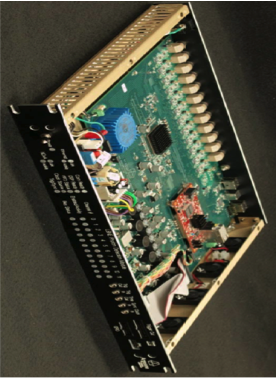
\includegraphics[angle=90,width=0.41\textwidth]{fig-e-2.png} 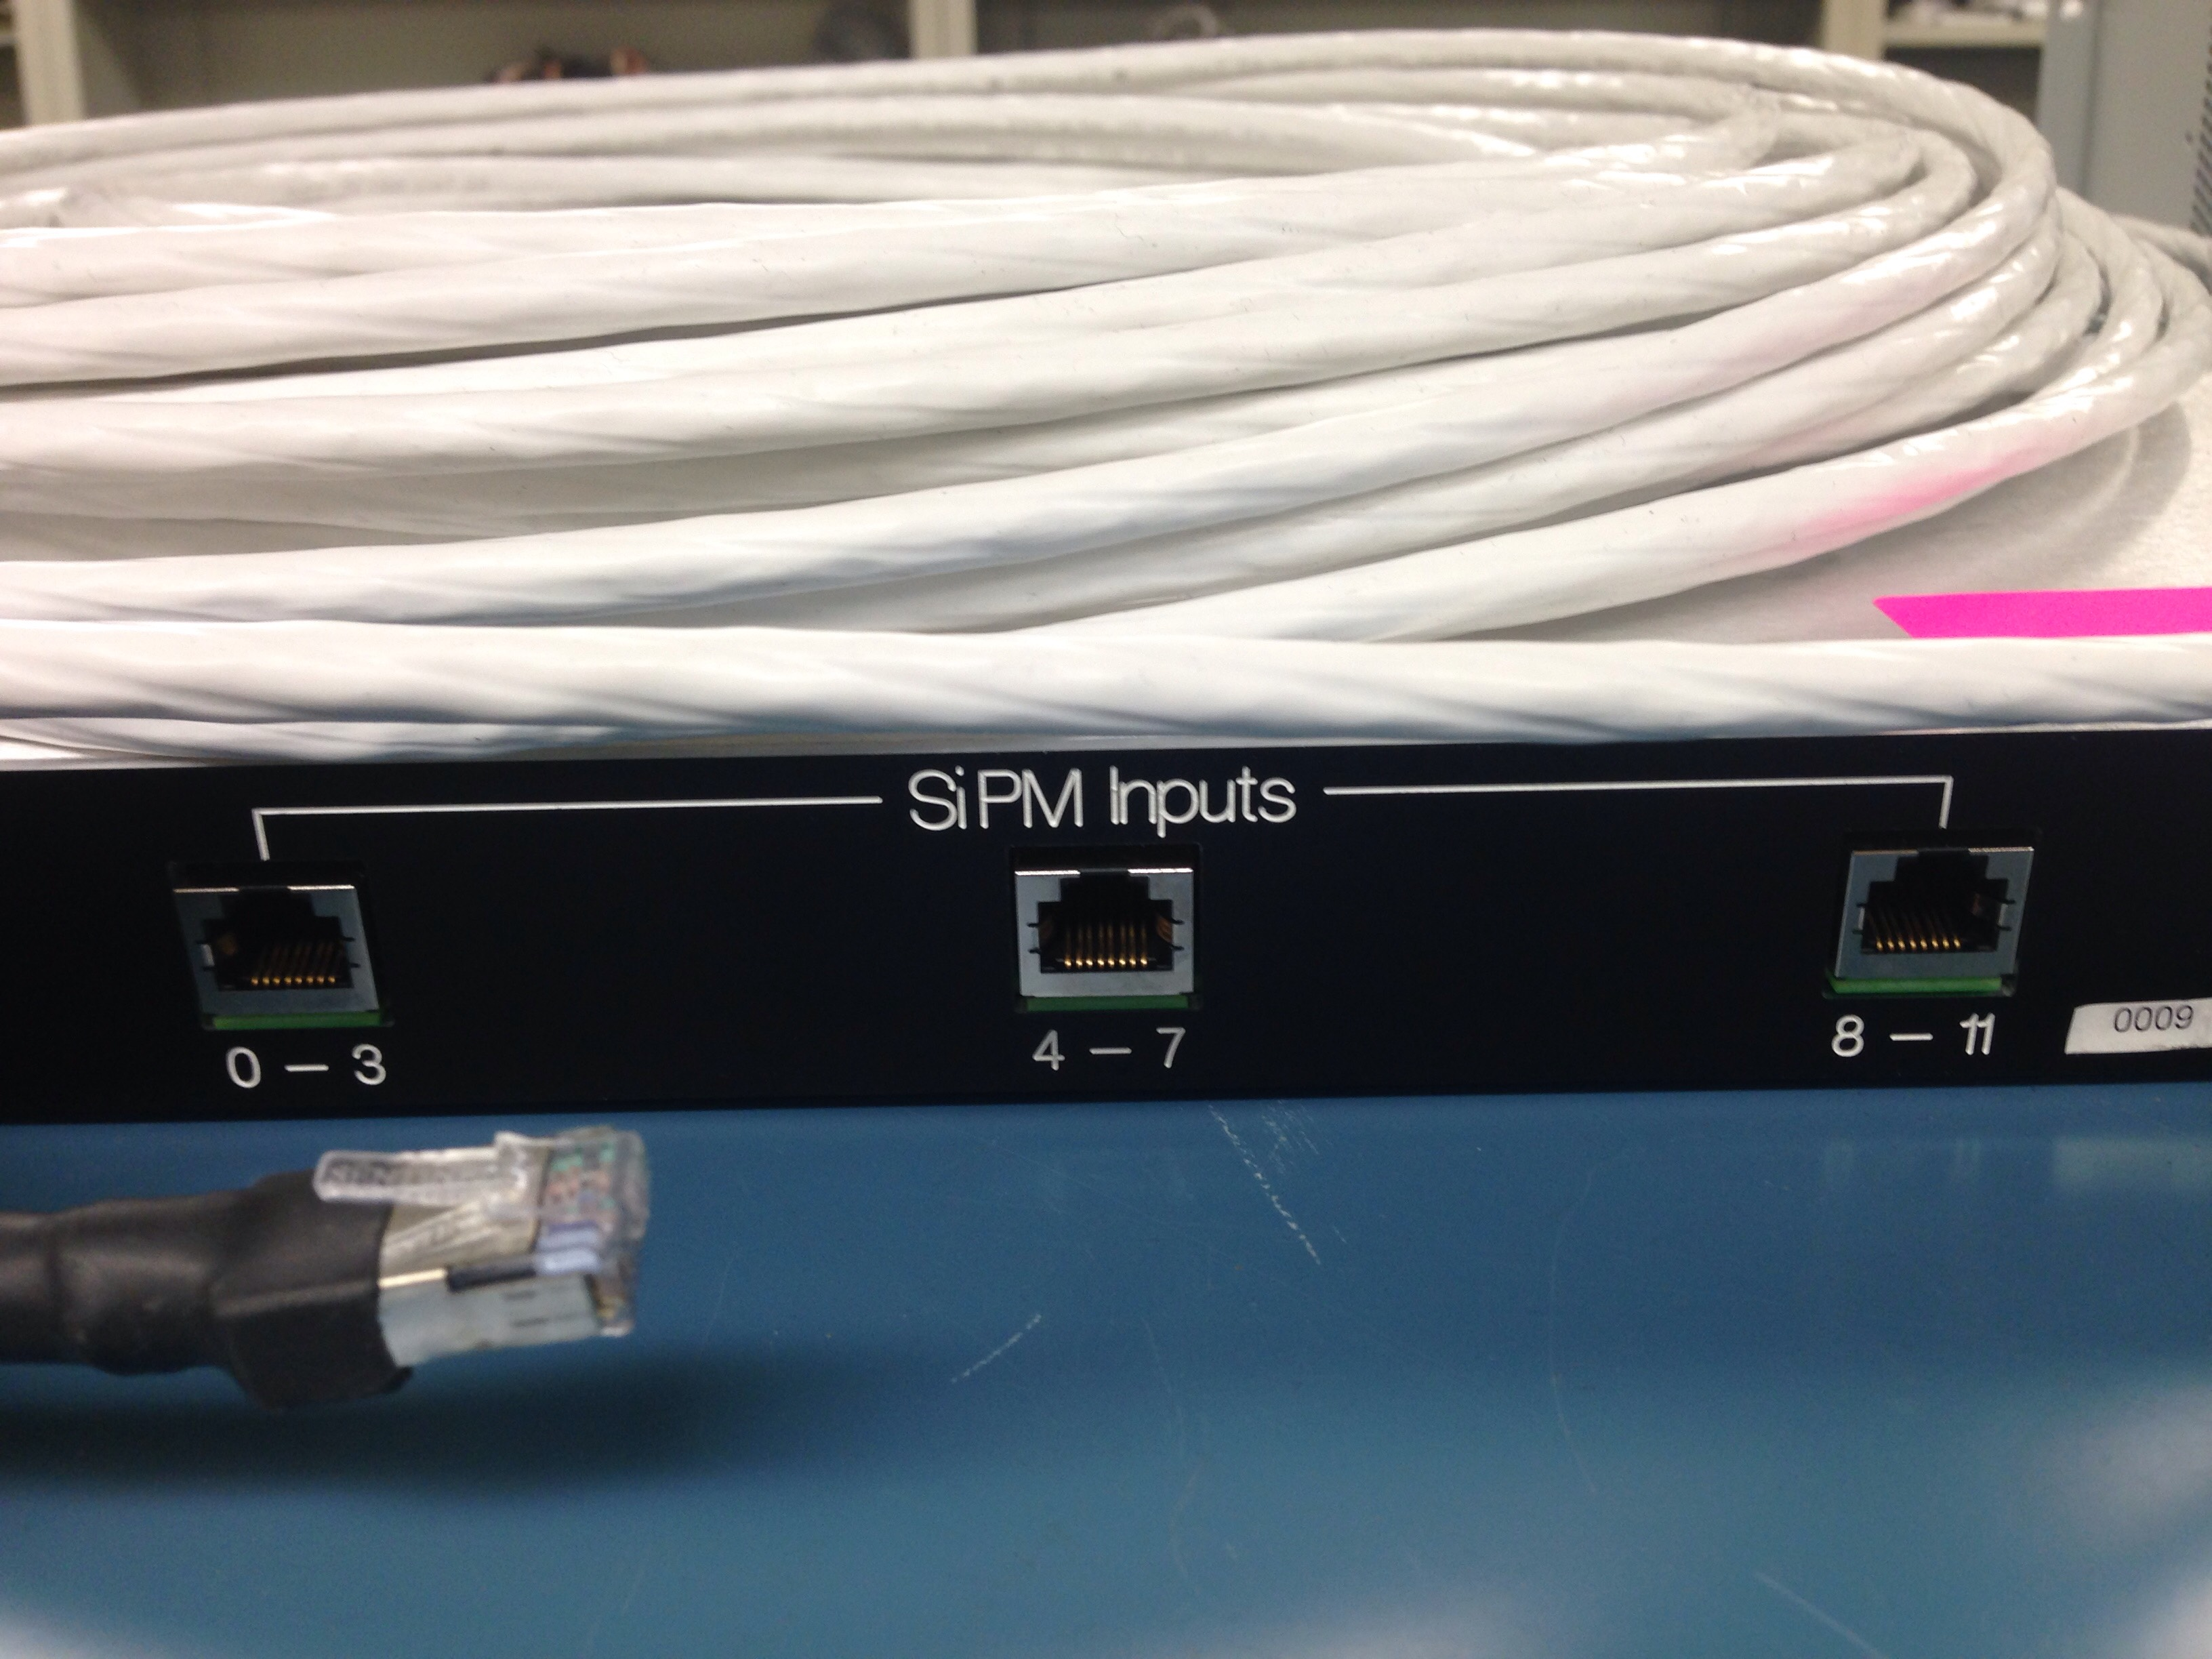
\includegraphics[angle=0,width=0.4\textwidth]{fig-ssp-cat6.jpg}
%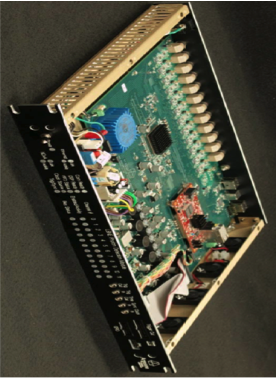
\includegraphics[angle=90,width=6.5cm,height=5cm]{fig-e-2.png} 
%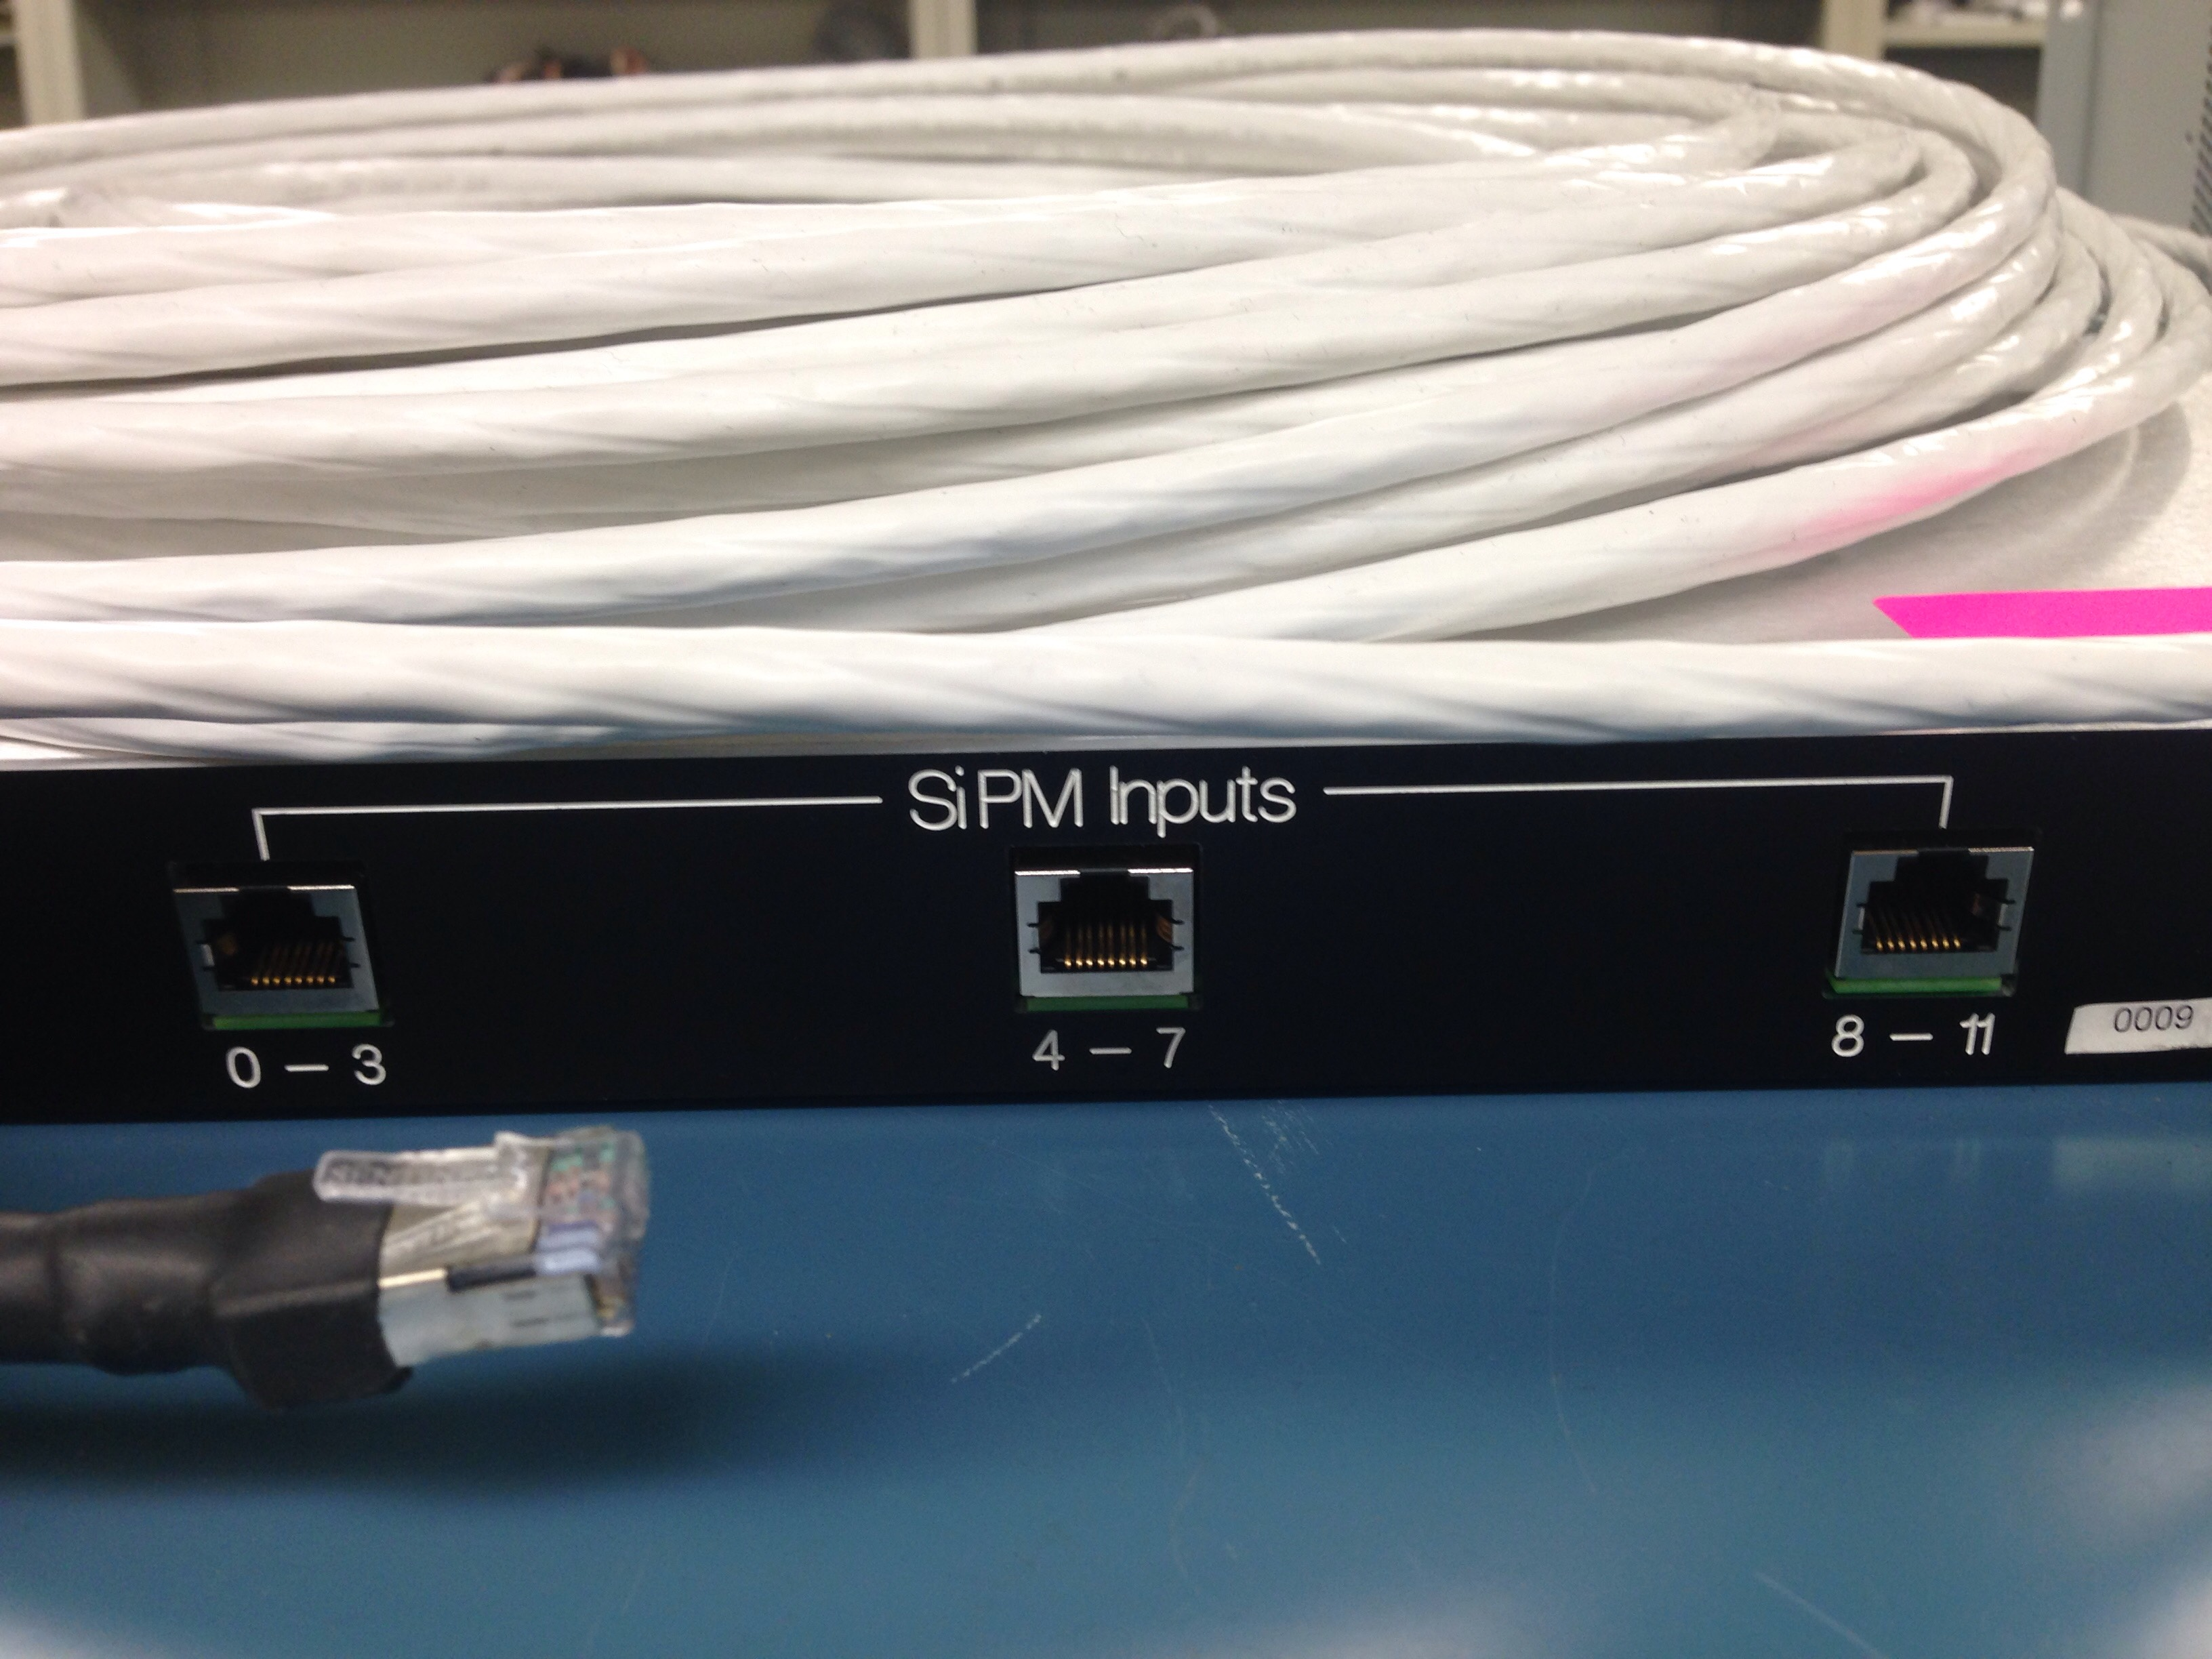
\includegraphics[angle=0,width=6.5cm,height=5cm]{fig-ssp-cat6.jpg}
\end{cdrfigure}
%
%Fig. xx2.  Block diagram of the SSP.

In order for the events measured in the photon detector to be matched up 
with the corresponding events in the TPC, the front-end electronics 
attaches a timestamp to the data as it is acquired.  
The timestamp is unique, and has a correspondence with the timestamps in 
the TPC electronics processing.  
The timestamp in the SSP is applied to the event data as it is digitized. 
%In the case where zero-suppression and data sparsification are used, 
%the timestamp on accepted data remains intact.  
To achieve this, the TPC and PD electronics must be synchronized, 
including timestamp counter resets, based on a known and stable calibration 
for the timing resolution of the ADC conversion between the two systems.  
In the ProtoDUNE-SP the photon readout is configured to read waveforms when triggered by a beam event,
and/or to provide header information when self-triggered by cosmic muons.
The header portion summarizes pulse amplitude, integral, and time-stamp information of events.
%and will capture times over threshold of waveforms, and will capture the timestamp of the event. 

A Xilinx Zynq FPGA handles the slow control and event data transfer.  
The SSP for ProtoDUNE-SP uses Gb Ethernet communication implemented over an optical interface.
The 1 Gb/s Ethernet supports full TCP/IP protocol.  
The module includes a separate 12-bit high-voltage DAC for each channel to 
provide up to 30\,V of bias to each SiPM.  
The module also features charge injection for performing diagnostics and linearity 
monitoring, and also voltage monitoring.

In tests to date, the SSP has been able to measure single photo-electron signals 
coming from the SiPMs over a cable length of 25 meters, when three SiPMs 
are summed together and operated at LAr temperatures.  
The timing resolution of the signals has been measured to be better than 3\,ns.  
The full-differential signal processing in the front-end circuitry 
is important in achieving this result.

The SSP provides a trigger output signal from internal discriminators in firmware based on programmable
coincidence logic, with a standard ST fiber interface to the central trigger board (CTB).
Input signals are provided to CTB from the beam instrumentation, the SSPs, and the beam TOF system.
The CTB receives timing information from the ProtoDUNE-SP timing system and the CTB trigger inputs are distributed to 
the experiment via the timing system.
To that end the SSP implements the timing receiver/transmitter endpoint hardware to receive trigger inputs and clock \fixme{signals?} from the timing system.
A block diagram of the system is shown in Figure~\ref{fig:PD_fig-e-3}.
%
\begin{cdrfigure}[Block diagram of the ProtoDUNE SSP module]{PD_fig-e-3}{Block diagram of the ProtoDUNE SSP module} 
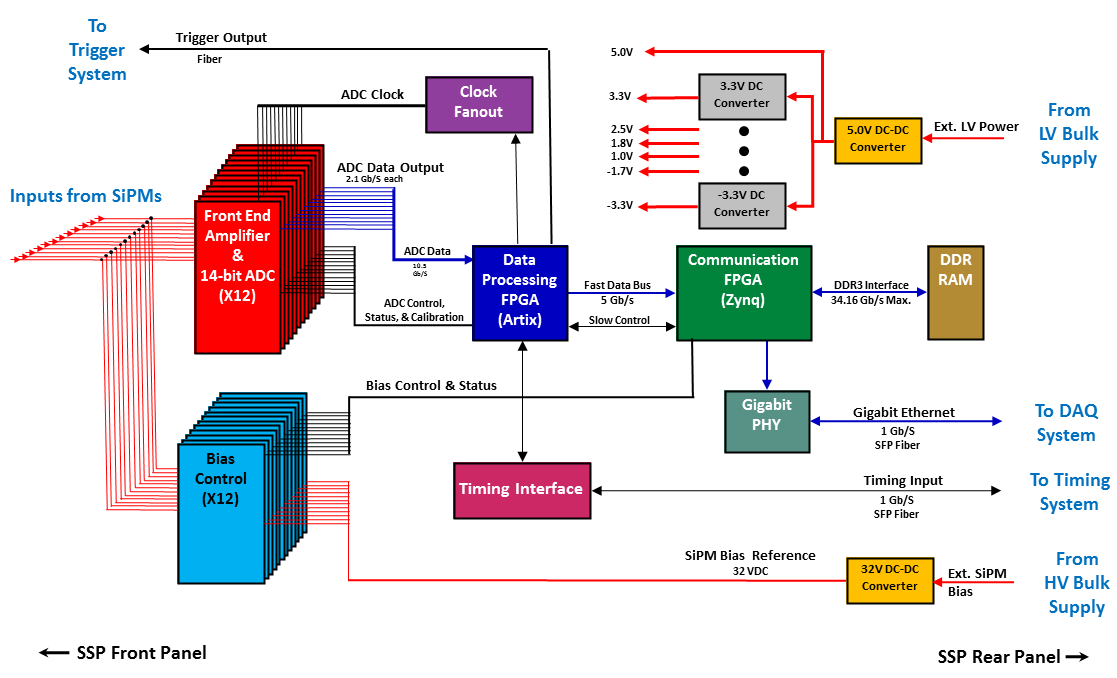
\includegraphics[width=\textwidth]{ProtoDUNE-SSP-block-diagram.png}
%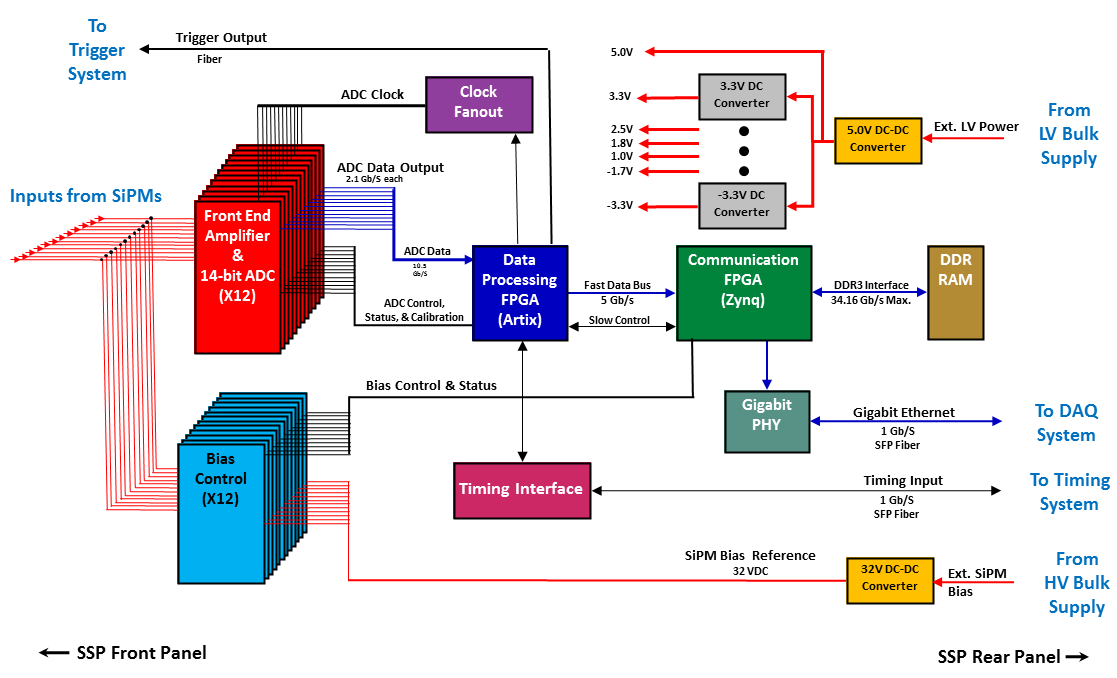
\includegraphics[angle=0,width=14cm,height=9cm]{ProtoDUNE-SSP-block-diagram.png}
\end{cdrfigure}
